\uuid{Ak8J}
\exo7id{4993}
\titre{exo7 4993}
\auteur{quercia}
\organisation{exo7}
\datecreate{2010-03-17}
\isIndication{false}
\isCorrection{true}
\chapitre{Courbes planes}
\sousChapitre{Coordonnées polaires}
\module{Géométrie}
\niveau{L2}
\difficulte{}

\contenu{
\texte{
Construire les courbes en polaires suivantes :
}
\begin{enumerate}
    \item \question{$\rho=\dfrac{\cos\theta/2}{1+\sin\theta}$                     \par
% \vtop to 7cm{\mapleplot{% 				img14
% r:=cos(t/2)/(1+sin(t));
% print(plot([r,t,t=0..4*Pi],view=[-2.8..2.8,-2..2],coords=polar));}   \par
% \vss}}
\reponse{$$
\centerline{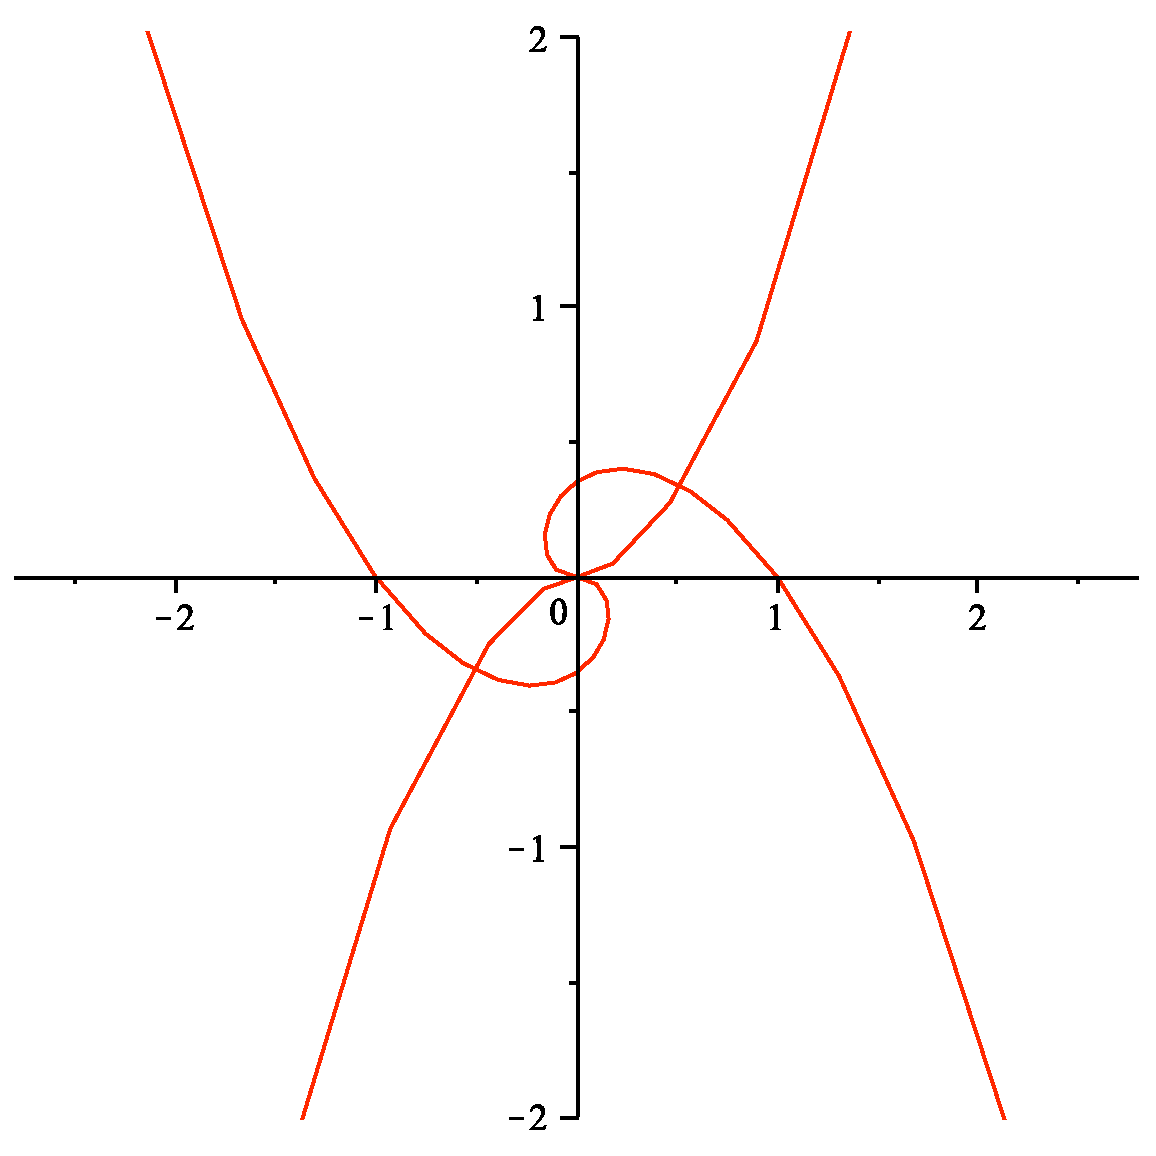
\includegraphics[height=4cm]{../images/pdf/Ak8J-1.pdf}}
$$}
    \item \question{$\rho=\dfrac{\cos2\theta}\cos\theta$                          \par
% \vtop to 7cm{\mapleplot{% 				img15
% r:=cos(2*t)/cos(t);
% print(plot([r,t,t=-Pi/2..Pi/2],view=[-2..2,-2..2],coords=polar));}   \par
% \vss}}
\reponse{$$
\centerline{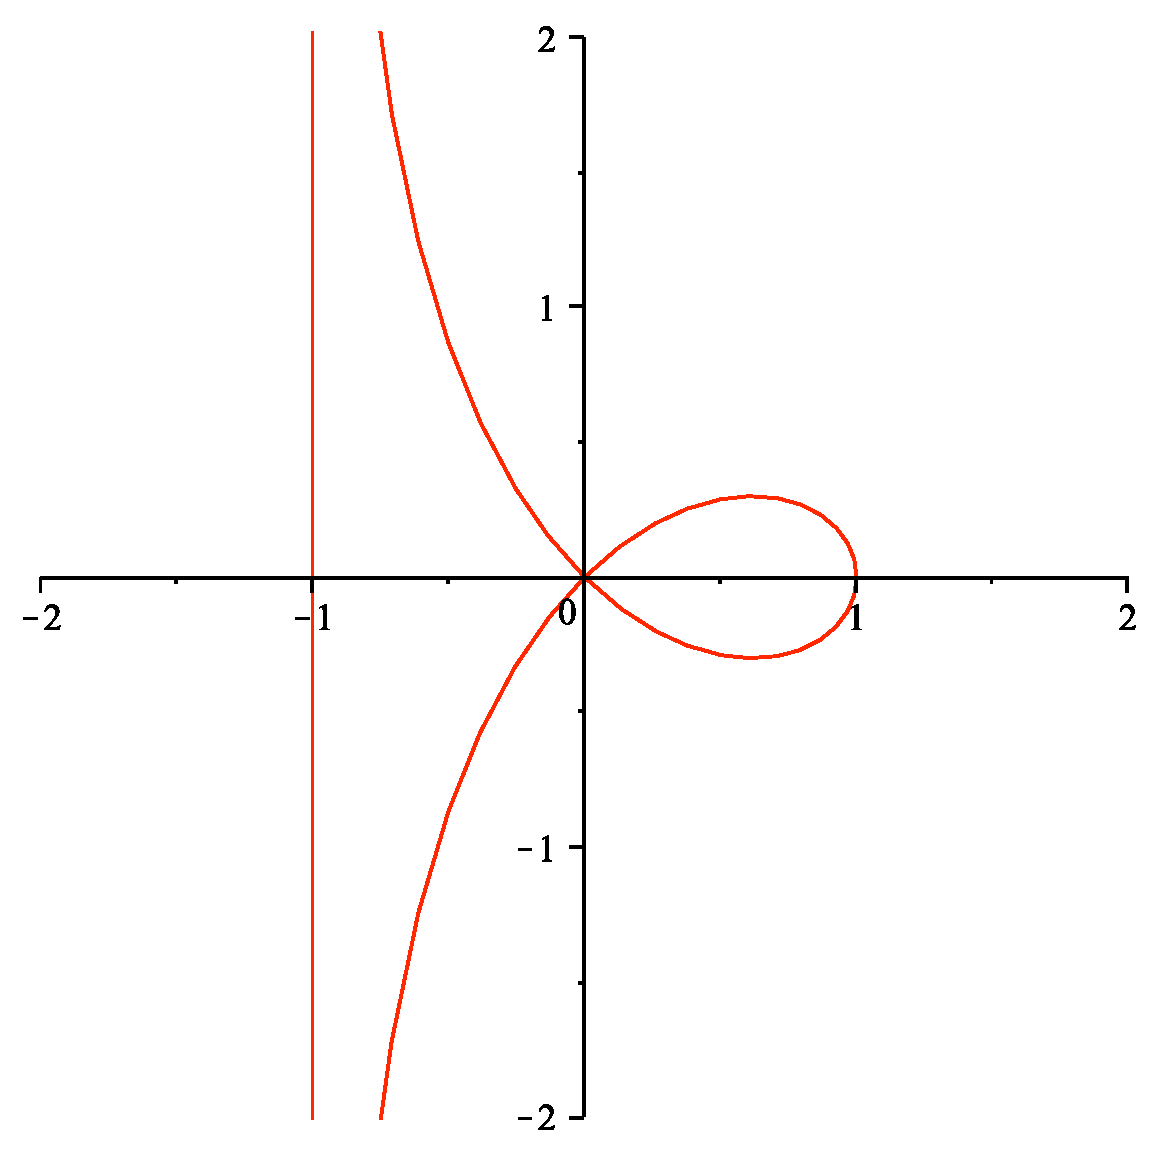
\includegraphics[height=4cm]{../images/pdf/Ak8J-2.pdf}}
$$
aire de la boucle : $2-\dfrac\pi2$                            \par}
    \item \question{$\rho=\dfrac{\sin\theta}{2\cos\theta-1}$                      \par
% \vtop to 7cm{\mapleplot{%				img16
% r:=sin(t)/(2*cos(t)-1);
% print(plot([r,t,t=-Pi..Pi],view=[-2..2,-3..1],coords=polar));}       \par
% \vss}}
\reponse{$$
\centerline{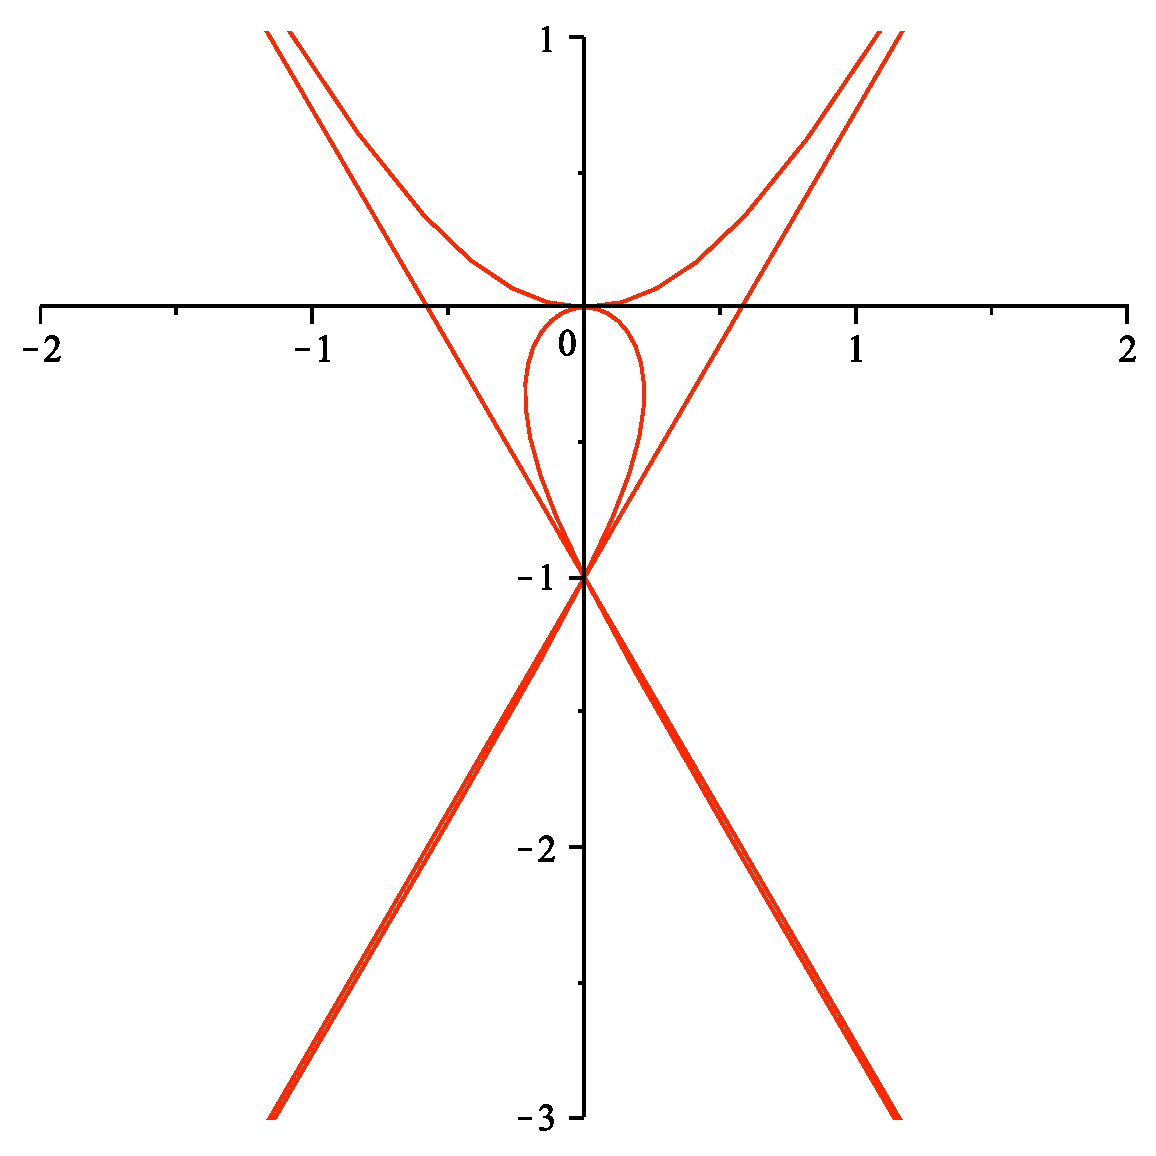
\includegraphics[height=4cm]{../images/pdf/Ak8J-3.pdf}}
$$
asymptotes : $y=\pm x\sqrt3-1$                                \par
la courbe traverse ses asymptotes au point de concours        \par}
    \item \question{$\rho=\dfrac1{\cos\theta+\sin2\theta}$                        \par
% \vtop to 7cm{\mapleplot{%				img17
% r:=1/(cos(t)+sin(2*t));
% print(plot([r,t,t=-Pi..Pi],view=[-4..4,-3..3],coords=polar));}       \par
% \vss}}
\reponse{$$
\centerline{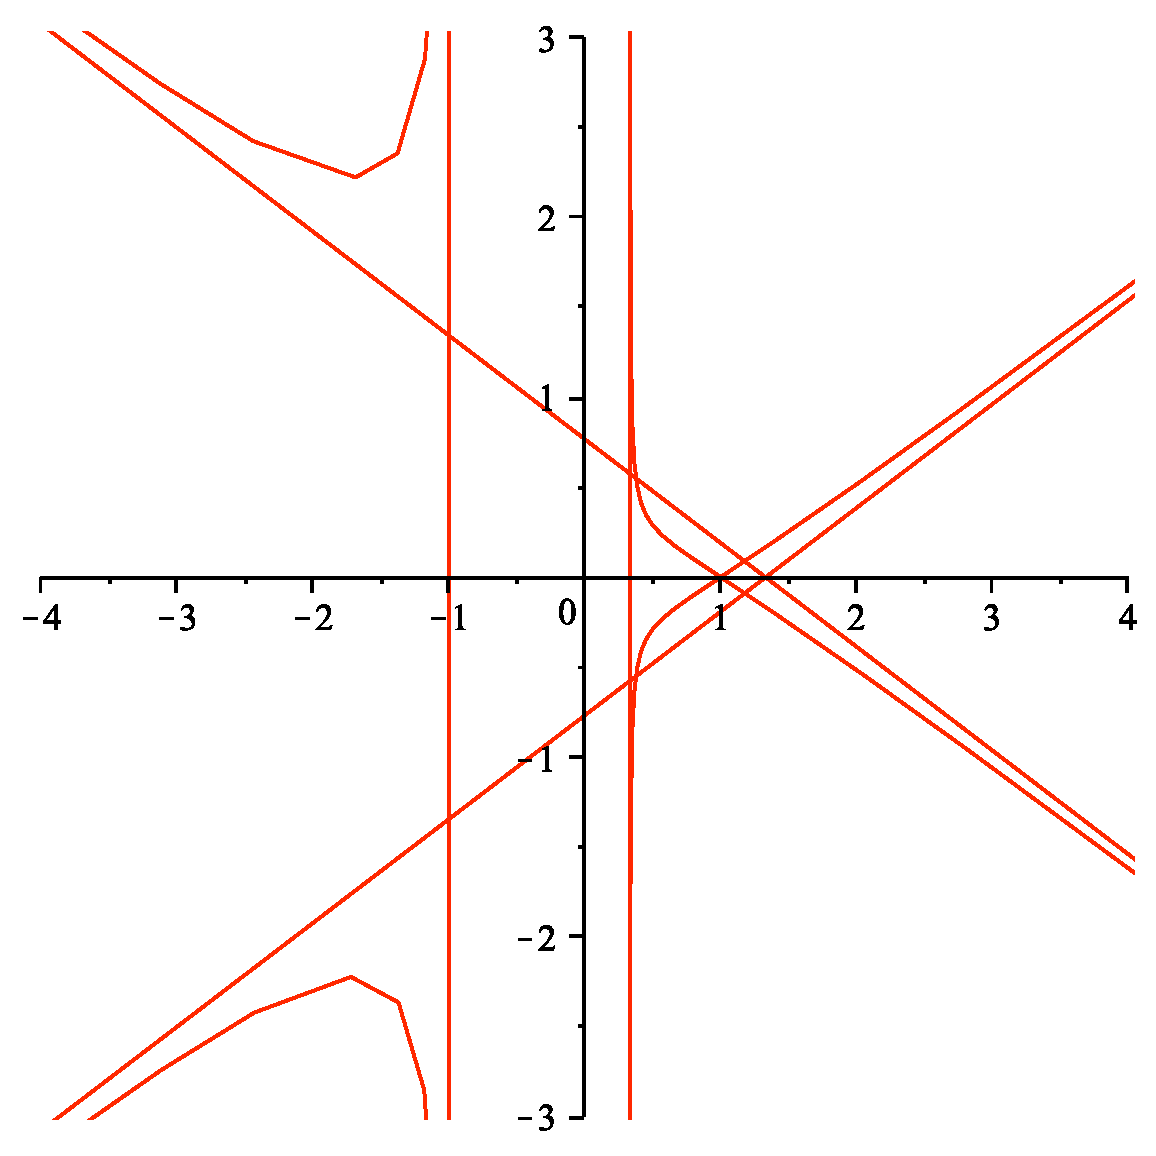
\includegraphics[height=4cm]{../images/pdf/Ak8J-4.pdf}}
$$
asymptotes : $x\pm y\sqrt3=\dfrac43$                           \par}
    \item \question{$\rho=\cos\theta+\dfrac1\cos\theta$                           \par
% \vtop to 7cm{\mapleplot{%				img18
% r:=cos(t)+1/cos(t);
% print(plot([r,t,t=-Pi/2..Pi/2],view=[0..3,-5..5],coords=polar));}    \par
%
% \vss}}
\reponse{$$
\centerline{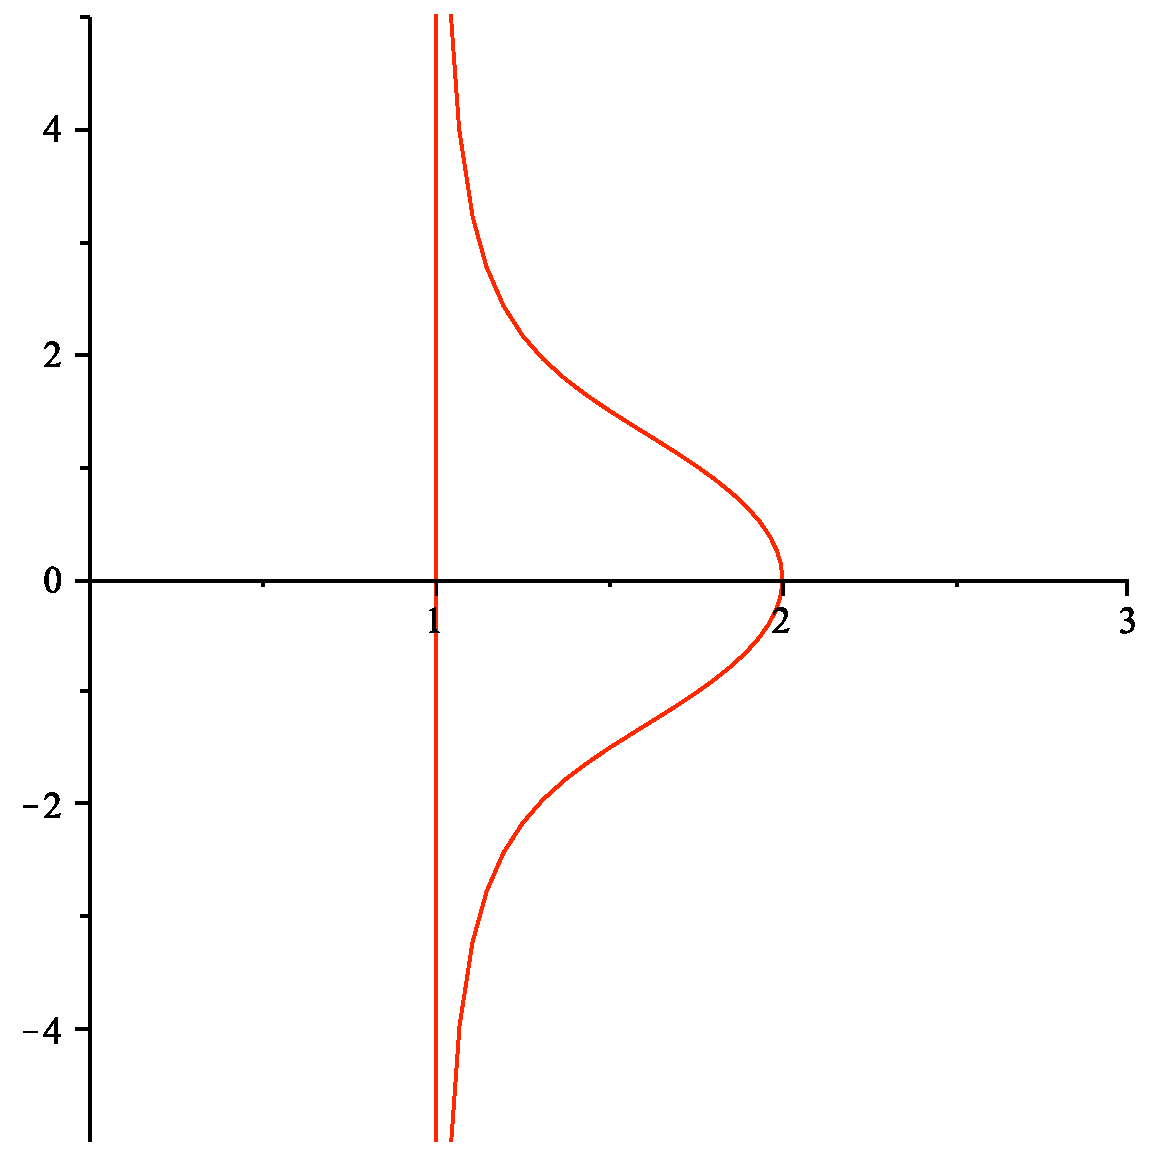
\includegraphics[height=4cm]{../images/pdf/Ak8J-5.pdf}}
$$}
    \item \question{$\rho=\dfrac{\cos2\theta}{2\cos\theta-1}$                     \par

% \vtop to 7cm{\mapleplot{%				img19
% r:=cos(2*t)/(2*cos(t)-1);
% print(plot([r,t,t=-Pi..Pi],view=[-2..2,-2..2],coords=polar));}       \par
% \vss}
%}
\reponse{$$
\centerline{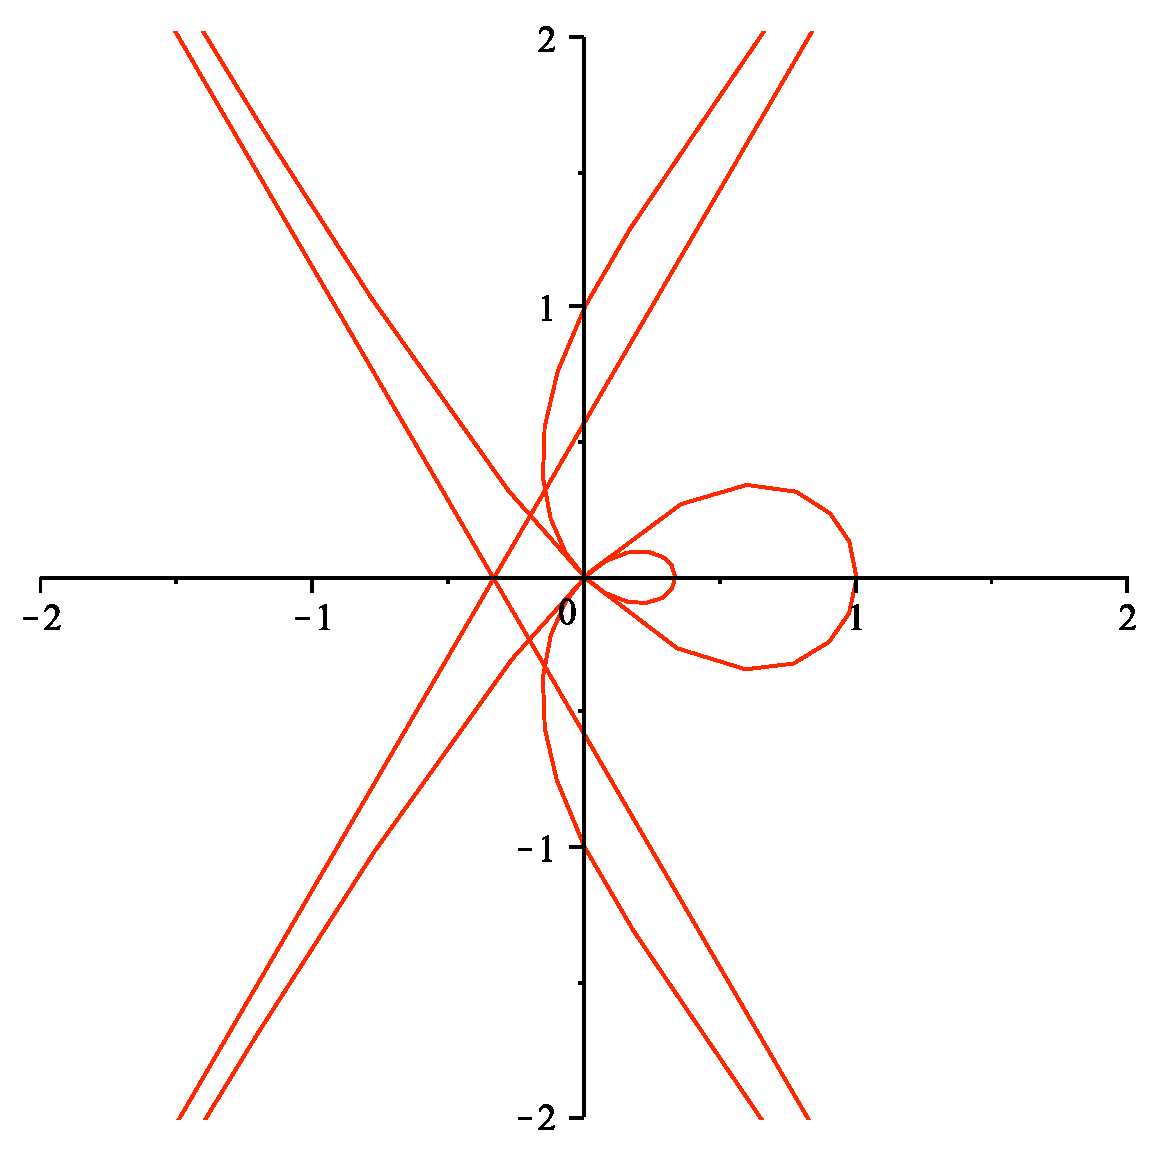
\includegraphics[height=4cm]{../images/pdf/Ak8J-6.pdf}}
$$
asymptotes : $3x\pm y\sqrt3=-1$                               \par}
    \item \question{$\rho=\cos\dfrac\theta3$                                                  \par
% \vtop to 7cm{\mapleplot{%				img20
% r:=cos(t/3);
% print(plot([r,t,t=0..6*Pi],scaling=constrained,coords=polar,axes=frame));}\par
% \vss}}
\reponse{$$
\centerline{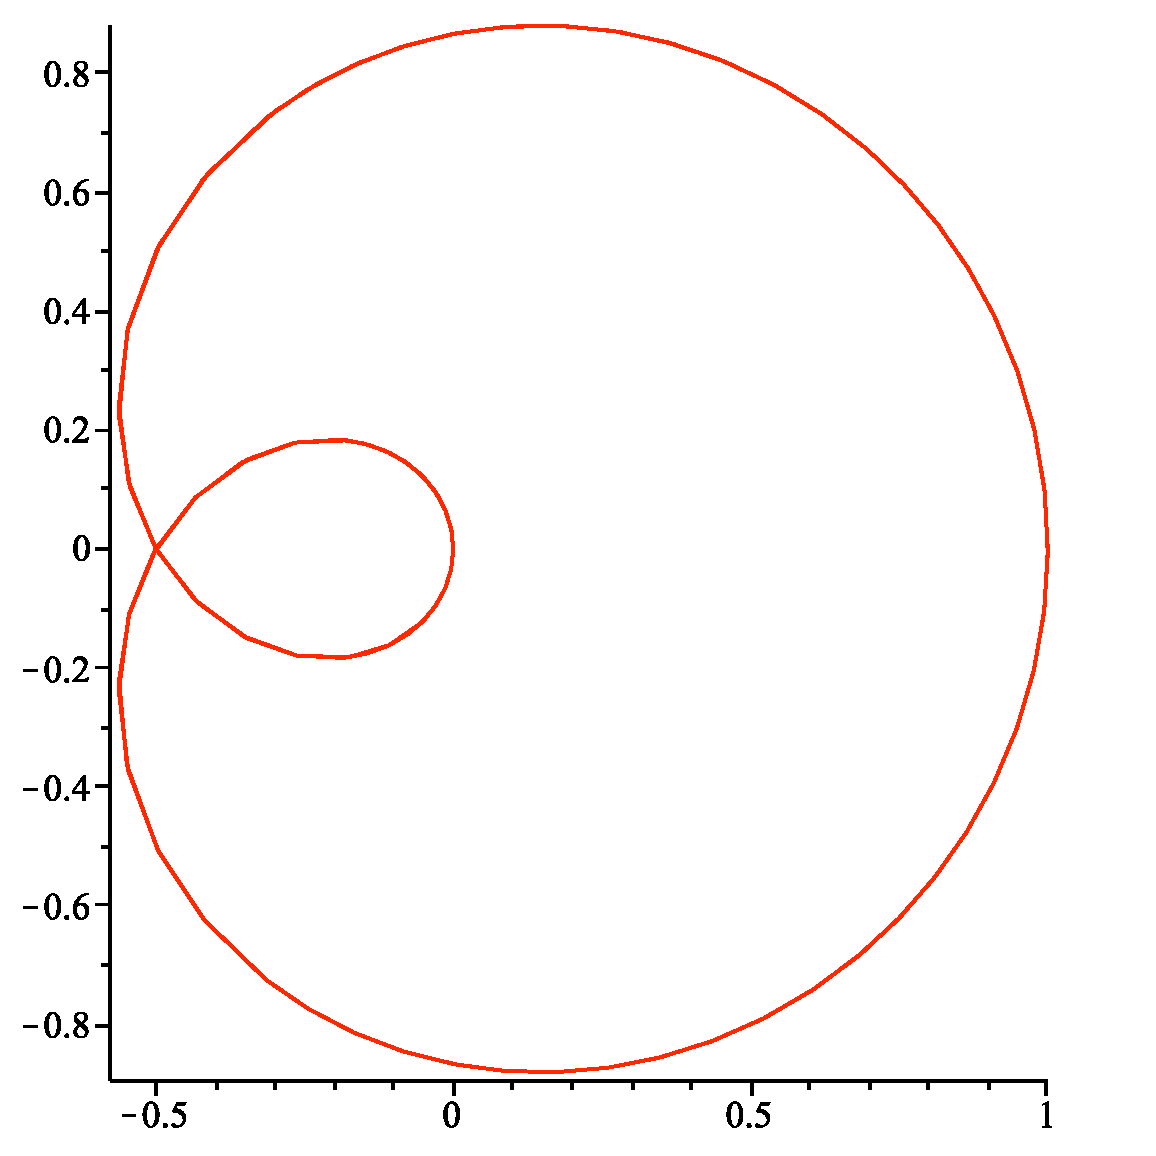
\includegraphics[height=4cm]{../images/pdf/Ak8J-7.pdf}}
$$}
    \item \question{$\rho=1+\sin3\theta$                                                      \par
% \vtop to 7cm{\mapleplot{%				img21
% r:=1+sin(3*t);
% print(plot([r,t,t=0..2*Pi],scaling=constrained,coords=polar,axes=frame));}\par
% \vss}}
\reponse{$$
\centerline{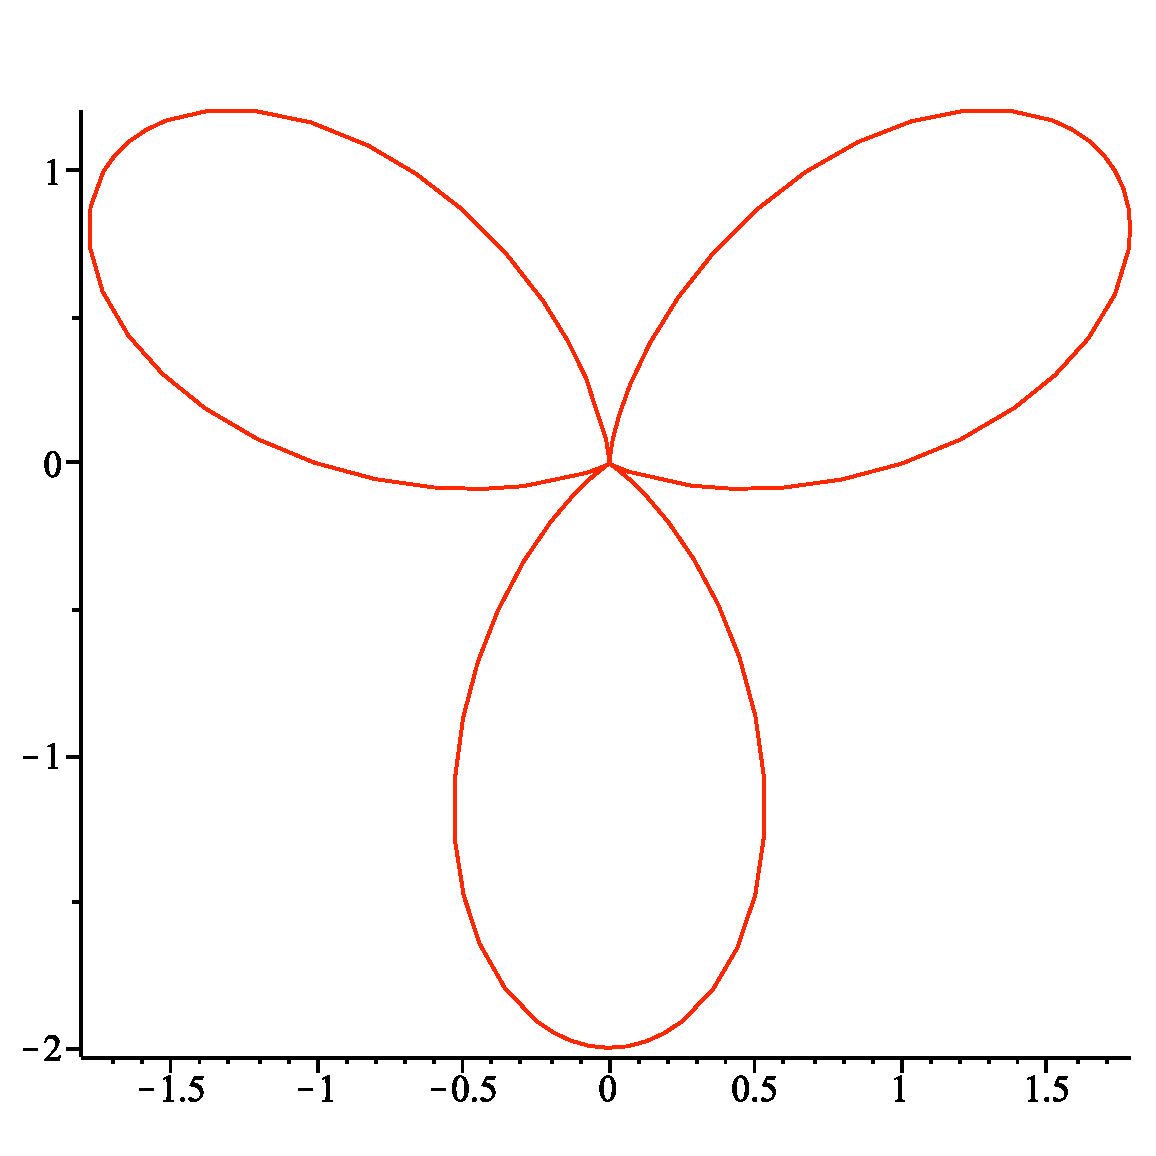
\includegraphics[height=4cm]{../images/pdf/Ak8J-8.pdf}}
$$}
    \item \question{$\rho=\dfrac1{\sqrt\theta}$                                   \par
% \vtop to 7cm{\mapleplot{%				img22
% r:=1/sqrt(t);
% print(plot([r,t,t=0..6*Pi],view=[-2..2,-1.4..1.4],coords=polar));}   \par
% \vss}}
\reponse{$$
\centerline{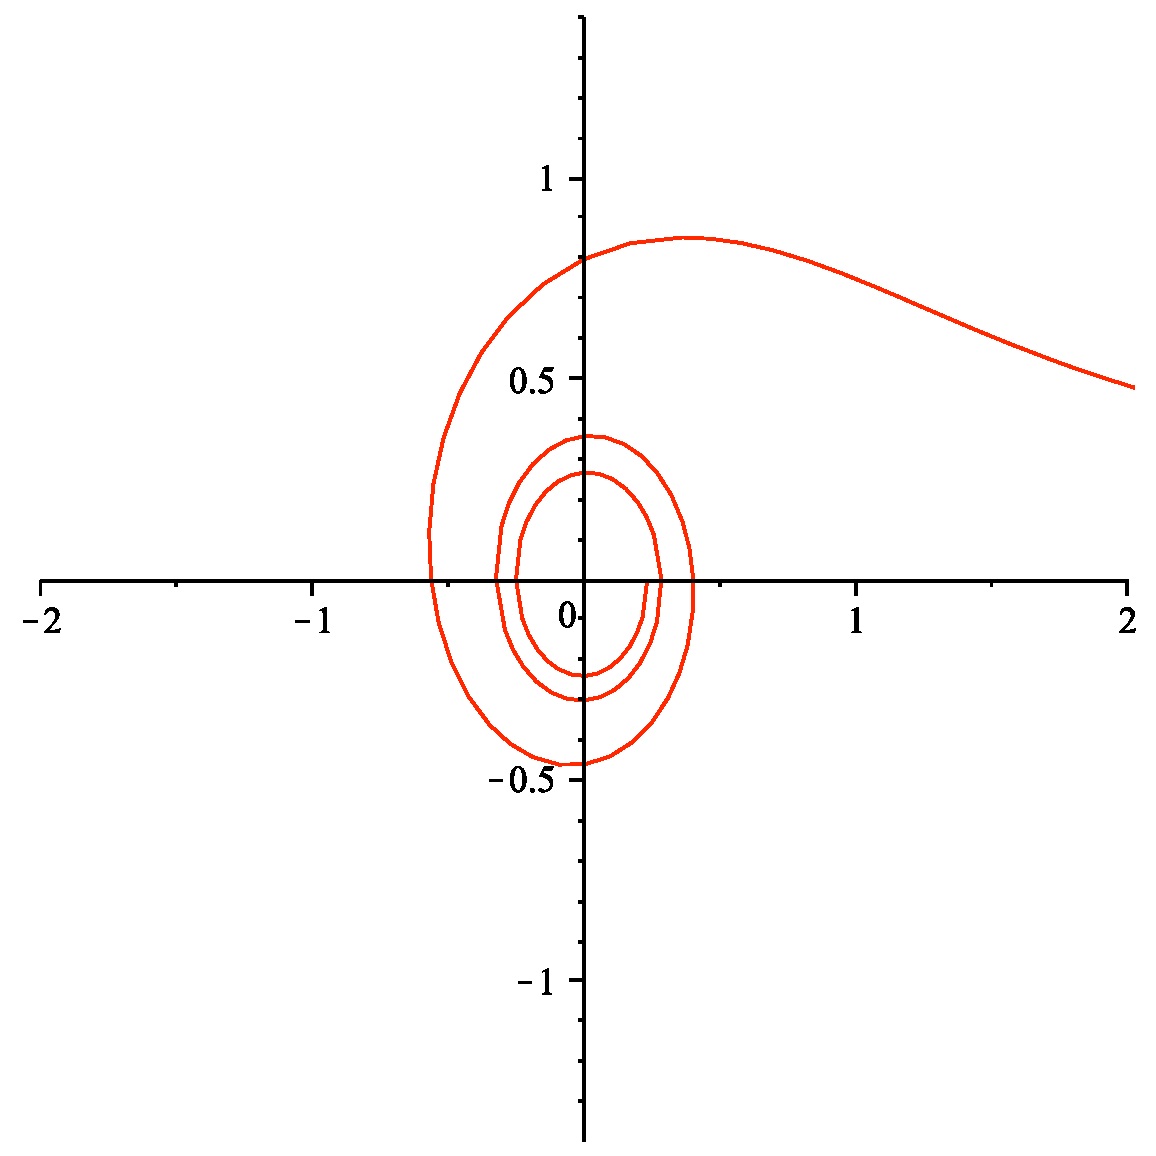
\includegraphics[height=4cm]{../images/pdf/Ak8J-9.pdf}}
$$}
    \item \question{$\rho=\ln\theta$                                              \par
% \vtop to 7cm{\mapleplot{%				img23
% r:=ln(t);
% print(plot([r,t,t=0..20],view=[-4..4,-3..3],coords=polar));}         \par
% \vss}}
\reponse{$$
\centerline{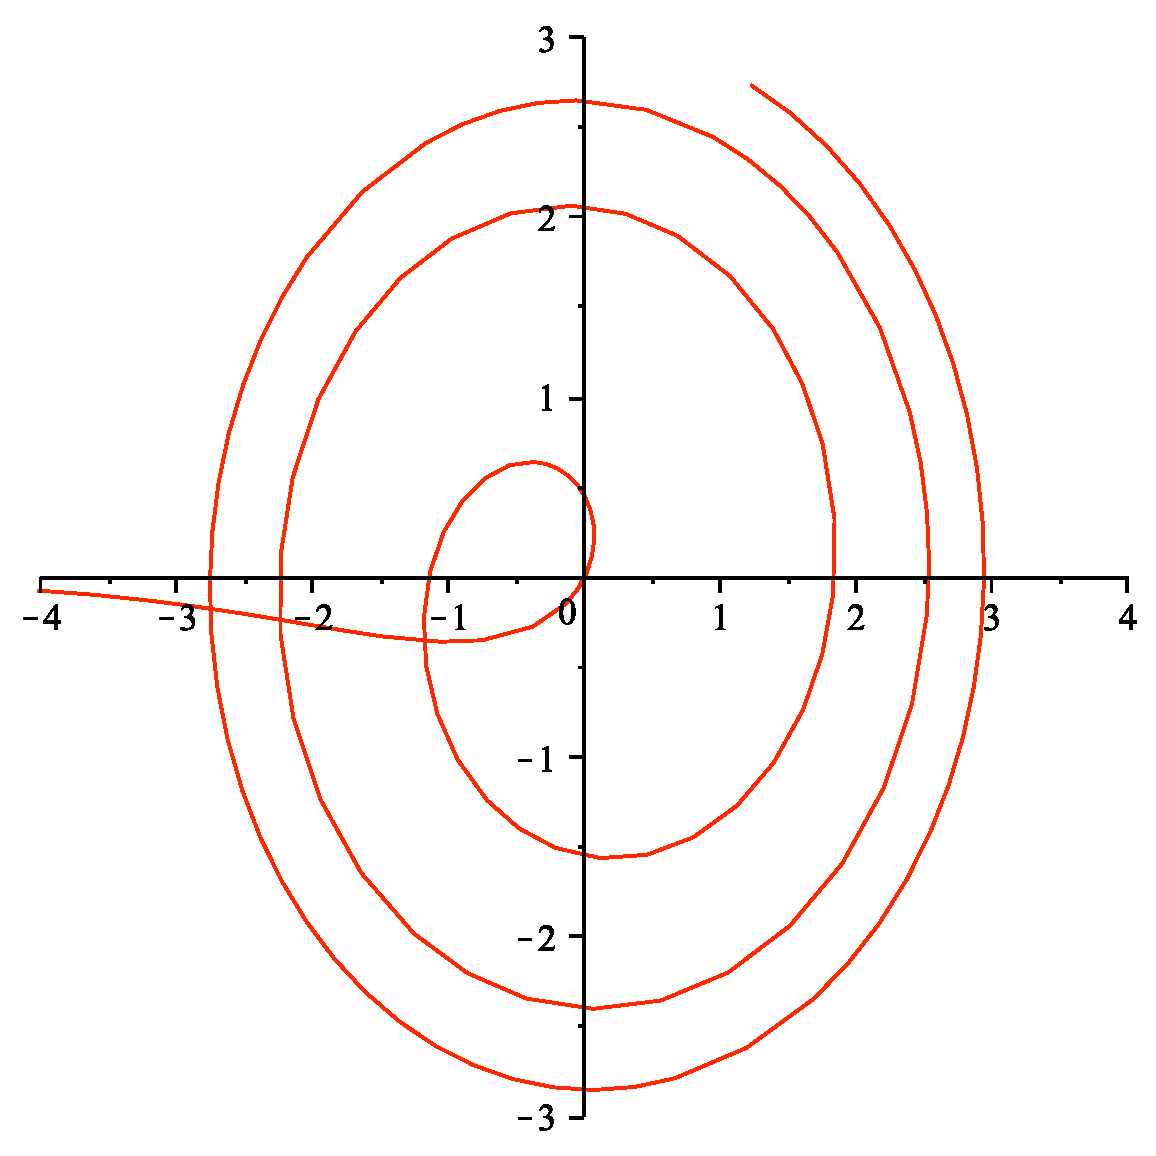
\includegraphics[height=4cm]{../images/pdf/Ak8J-10.pdf}}
$$}
    \item \question{$\rho=\frac{\sin\theta}\theta$                                               \par
% \vtop to 7cm{\mapleplot{%				img24
% r:=sin(t)/t;
% print(plot([r,t,t=-6*Pi..6*Pi],scaling=constrained,coords=polar,axes=frame));}\par
% \vss}
% 
%}
\reponse{$$
\centerline{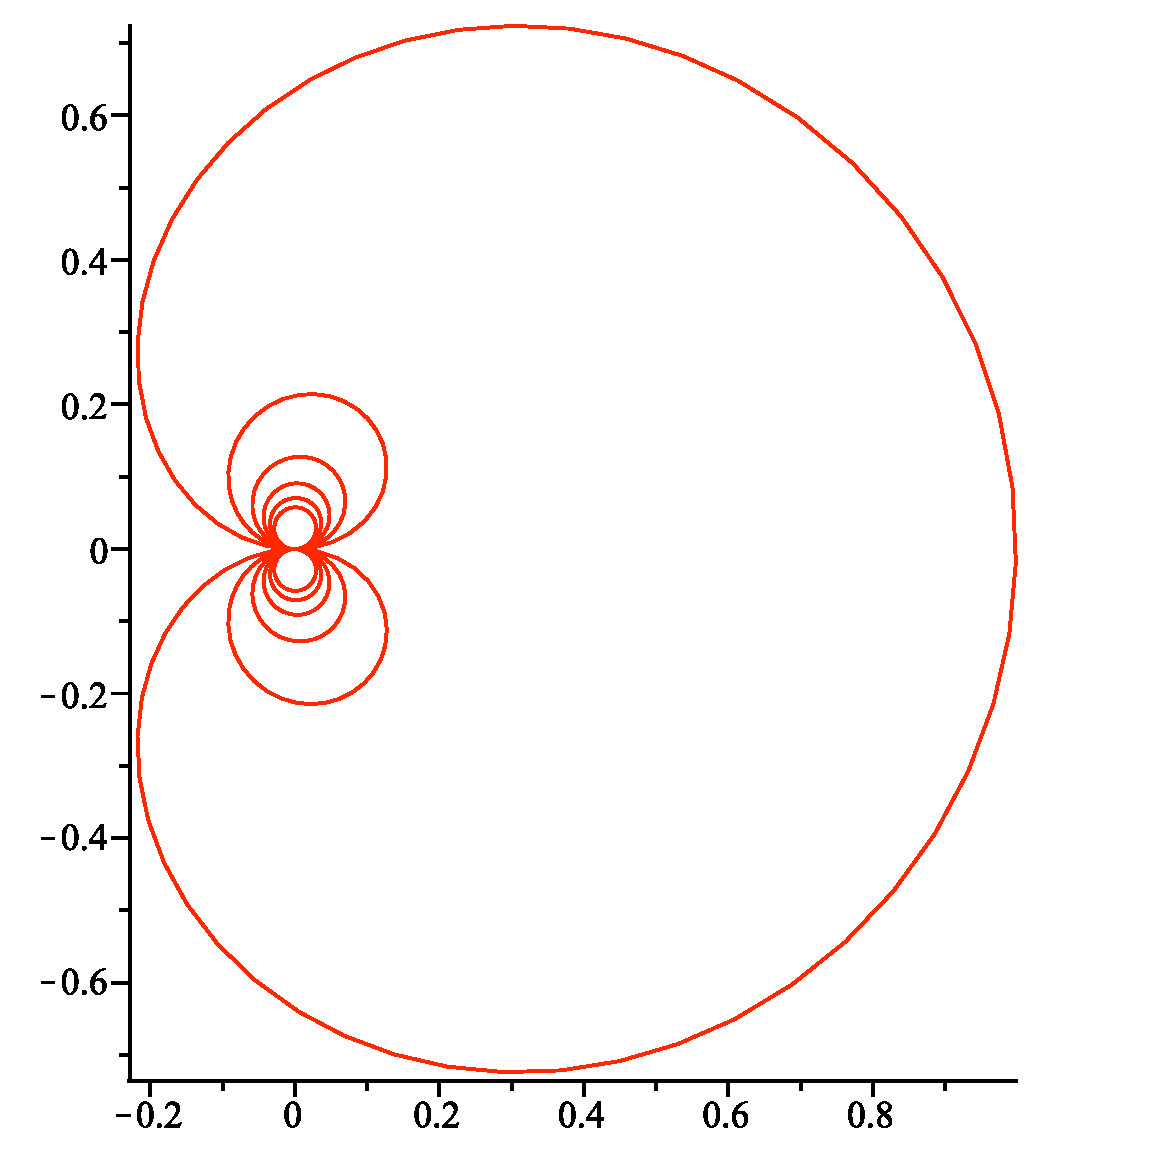
\includegraphics[height=4cm]{../images/pdf/Ak8J-11.pdf}}
$$}
\end{enumerate}
}
